%!TEX program = xelatex

\documentclass[11pt,titlepage]{report}
%!TEX root = main.tex

\usepackage[T1]{fontenc}
\usepackage{lmodern}
\usepackage[svgnames]{xcolor}
\usepackage{fontspec} % XeLaTeX required!
\usepackage{graphicx}
\usepackage{circuitikz}
\usepackage{tikz}
\usepackage{pifont}
\usepackage[some]{background}
\usepackage{xltxtra} 
\usepackage{setspace}
\usepackage[absolute]{textpos}
\usepackage[latin1]{inputenc}
\usepackage[english]{babel}
\usepackage{graphicx}
\usepackage{wrapfig}
\usepackage{fullpage}
\usepackage[margin=1in]{geometry}
\usepackage{float}
\usepackage{url}
\usepackage{multicol}
\usepackage{hyperref}
\usepackage{titlepic}
\usepackage{standalone}
\usepackage{siunitx}
\usepackage{booktabs}
\usepackage{amsmath}
\usepackage{unicode-math}
\usepackage{verbatim}
\usepackage{enumitem}
\usepackage{listings}
\usepackage{multirow}
\usepackage{pgfplots}
\pgfplotsset{compat=1.8}
\usepackage{caption} 
\usepackage[parfill]{parskip}
\usepackage{import}
\usepackage[backend=bibtexu,texencoding=utf8,bibencoding=utf8,style=ieee,sortlocale=en_GB,language=auto]{biblatex}
\usepackage[strict,autostyle]{csquotes}
\usepackage[final]{pdfpages}
\usepackage{subcaption}
\usepackage{ifplatform}
%\captionsetup[table]{skip=10pt}


% Fix for includepdf bug in Mac OS X
\newcommand{\insertpdfpath}[1]{
	\ifwindows
	\newcommand{\insertpdf}[2]{\includepdf[pages=##1]{##2}}
	\else
	\newcommand{\insertpdf}[2]{\includepdf[pages=##1]{#1/##2}}
	\fi
}

%set fonts
\setmainfont[Ligatures=TeX]{Myriad Pro}
\setmathfont{Asana Math}
\setmonofont{Lucida Console}

\usepackage{titlesec, color}
\renewcommand{\familydefault}{\sfdefault} %set font family
\renewcommand{\arraystretch}{1.2} %set table vertical spacing
\setlength\parindent{0pt} %no paragraph indent
\hypersetup{ %setup hyperlinks
    colorlinks,
    citecolor=black,
    filecolor=black,
    linkcolor=black,
    urlcolor=black
}

%redesign chapter headings
\definecolor{gray75}{gray}{0.75}
\newcommand{\chapternumber}{\thechapter}
\newcommand{\hsp}{\hspace{20pt}}
\titleformat{\chapter}[hang]{\Huge\bfseries}{\chapternumber\hsp\textcolor{gray75}{|}\hsp}{0pt}{\Huge\bfseries}

%Redefine appendix headers
\renewcommand{\appendixname}{Appendix}
\renewcommand{\appendixtocname}{Appendices}
\renewcommand{\appendixpagename}{Appendices}

%For code listings
\definecolor{black}{rgb}{0,0,0}
\definecolor{browntags}{rgb}{0.65,0.1,0.1}
\definecolor{bluestrings}{rgb}{0,0,1}
\definecolor{graycomments}{rgb}{0.4,0.4,0.4}
\definecolor{redkeywords}{rgb}{1,0,0}
\definecolor{bluekeywords}{rgb}{0.13,0.13,0.8}
\definecolor{greencomments}{rgb}{0,0.5,0}
\definecolor{redstrings}{rgb}{0.9,0,0}
\definecolor{purpleidentifiers}{rgb}{0.01,0,0.01}


\lstdefinestyle{csharp}{
language=[Sharp]C,
showspaces=false,
showtabs=false,
breaklines=true,
showstringspaces=false,
breakatwhitespace=true,
escapeinside={(*@}{@*)},
columns=fullflexible,
commentstyle=\color{greencomments},
keywordstyle=\color{bluekeywords}\bfseries,
stringstyle=\color{redstrings},
identifierstyle=\color{purpleidentifiers},
basicstyle=\ttfamily\small}

\lstdefinestyle{c}{
language=C,
showspaces=false,
showtabs=false,
breaklines=true,
showstringspaces=false,
breakatwhitespace=true,
escapeinside={(*@}{@*)},
columns=fullflexible,
commentstyle=\color{greencomments},
keywordstyle=\color{bluekeywords}\bfseries,
stringstyle=\color{redstrings},
identifierstyle=\color{purpleidentifiers},
}

\lstdefinestyle{matlab}{
language=Matlab,
showspaces=false,
showtabs=false,
breaklines=true,
showstringspaces=false,
breakatwhitespace=true,
escapeinside={(*@}{@*)},
columns=fullflexible,
commentstyle=\color{greencomments},
keywordstyle=\color{bluekeywords}\bfseries,
stringstyle=\color{redstrings},
identifierstyle=\color{purpleidentifiers}
}

\lstdefinestyle{vhdl}{
language=VHDL,
showspaces=false,
showtabs=false,
breaklines=true,
showstringspaces=false,
breakatwhitespace=true,
escapeinside={(*@}{@*)},
columns=fullflexible,
commentstyle=\color{greencomments},
keywordstyle=\color{bluekeywords}\bfseries,
stringstyle=\color{redstrings},
identifierstyle=\color{purpleidentifiers}
}

\lstdefinestyle{xaml}{
language=XML,
showspaces=false,
showtabs=false,
breaklines=true,
showstringspaces=false,
breakatwhitespace=true,
escapeinside={(*@}{@*)},
columns=fullflexible,
commentstyle=\color{greencomments},
keywordstyle=\color{redkeywords},
stringstyle=\color{bluestrings},
tagstyle=\color{browntags},
morestring=[b]",
  morecomment=[s]{<?}{?>},
  morekeywords={xmlns,version,typex:AsyncRecords,x:Arguments,x:Boolean,x:Byte,x:Char,x:Class,x:ClassAttributes,x:ClassModifier,x:Code,x:ConnectionId,x:Decimal,x:Double,x:FactoryMethod,x:FieldModifier,x:Int16,x:Int32,x:Int64,x:Key,x:Members,x:Name,x:Object,x:Property,x:Shared,x:Single,x:String,x:Subclass,x:SynchronousMode,x:TimeSpan,x:TypeArguments,x:Uid,x:Uri,x:XData,Grid.Column,Grid.ColumnSpan,Click,ClipToBounds,Content,DropDownOpened,FontSize,Foreground,Header,Height,HorizontalAlignment,HorizontalContentAlignment,IsCancel,IsDefault,IsEnabled,IsSelected,Margin,MinHeight,MinWidth,Padding,SnapsToDevicePixels,Target,TextWrapping,Title,VerticalAlignment,VerticalContentAlignment,Width,WindowStartupLocation,Binding,Mode,OneWay,xmlns:x}
}

\lstdefinestyle{matlab}{
language=Matlab,
showspaces=false,
showtabs=false,
breaklines=true,
showstringspaces=false,
breakatwhitespace=true,
escapeinside={(*@}{@*)},
columns=fullflexible,
commentstyle=\color{greencomments},
keywordstyle=\color{bluekeywords}\bfseries,
stringstyle=\color{purpleidentifiers},
identifierstyle=\color{purpleidentifiers}
}

%defaults
\lstset{
basicstyle=\ttfamily\small,
extendedchars=false,
numbers=left,
numberstyle=\ttfamily\tiny,
stepnumber=1,
tabsize=4,
numbersep=5pt
}
\addbibresource{../../library/bibliography.bib}

\begin{document}

\chapter{Assignment 1}
\section{Task 1}
Let us investigate the characteristic impedance $Z_0$, cutoff frequency $w_0$ and propagation coefficient $\gamma$ for a ladder network characterized by $Z_s=1/j \omega C$ and $Z_p=j \omega L$. The characteristic impedance is given by
\begin{align}
	Z_0 = \frac{Z_s}{2} + \sqrt{\frac{Z_s^2}{4} + Z_s Z_p}.
\end{align}

The propagation coefficient is given by
\begin{align}
	\gamma &= 1 - \frac{Z_s}{Z_0} \nonumber \\
	&= \frac{Z_0-Z_s}{Z-s} \nonumber \\
	&= \frac{\frac{Z_s}{2} + \sqrt{\frac{Z_s^2}{4} + Z_s Z_p}}{\frac{Z_s}{2} + \sqrt{\frac{Z_s^2}{4} + Z_s Z_p}} \nonumber \\
	&= \frac{-1 + 2j\sqrt{\frac{-1}{4} + w^2 L C}}{1 + 2j\sqrt{\frac{-1}{4} + \omega{}^2 L C}}.
\end{align}

For
\begin{align}
	0 &< \frac{-1}{4} + \omega^2 L C,  \nonumber \\
	\omega &> \frac{1}{2\sqrt{LC}} = \omega_0,
\end{align}

the length of $\gamma$ reduces to
\begin{align} \label{eq:ass-1-prop-higher}
	|\gamma| &= \sqrt{\frac{(-1)^2 + 4(\frac{-1}{4}+\omega^2 L C)}{1^2 + 4(\frac{-1}{4}+\omega^2 L C)}} = 1.
\end{align}

However, for $\omega<\omega_0$, $|\gamma|$ yields for some $X \in \mathbb{R}$, $X > 0$ 
\begin{align} \label{eq:ass-1-prop-lower}
	|\gamma| = \left|\frac{-1 + X}{1 + X}\right| < 1.
\end{align}

Equation \ref{eq:ass-1-prop-lower} and \ref{eq:ass-1-prop-higher} make clear that our signal, above a certain frequency, is not damped anymore ($\gamma=1$). Therefore, our ladder network behaves as a high-pass filter.

\section{Task 2}
The reflection coefficient $\Gamma$ is given by
\begin{equation}
	\Gamma = \frac{Z_l - Z_0}{Z_l + Z_0}.
\end{equation}

We see that when $Z_l \to 0$, $\Gamma \to -1$ and that when $Z_l \to \infty$, $\Gamma \to 1$. Therefore, the space-time expression of the voltage across the channel whose terminals are shorted, is given by
\begin{equation} \label{eq:ass-1-node}
	V(z,t)=U(t- \gamma z) - U(t+ \gamma(z-2l)) + U (t- \gamma(z + 2l)) -U(t + \gamma (z-4l)) + \dots
\end{equation}

In a same manner, the space-time expression of the voltage across the channel which is terminated by a very large load, is given by
\begin{equation} \label{eq:ass-1-anti-node}
	V(z,t)=U(t- \gamma z) + U(t+ \gamma(z-2l)) - U (t- \gamma(z + 2l)) - U(t + \gamma (z-4l)) + \dots
\end{equation}

Comparing Equation \ref{eq:ass-1-node} and \ref{eq:ass-1-anti-node} reveals that at the moment of reflection, \textbf{(1)}, for shorted terminals the polarity of the wave changes, and \textbf{(2)}, for open terminals the polarity of the wave remains the same. This makes sense, because shorted terminals can be considered a node, and open terminals an anti-node.

\section{Task 3}
Lets consider a $U(t)$ given by

\begin{equation}
	U(t) = V_{\text{max}}(\epsilon(t)-\epsilon(t-t_w)).
\end{equation}

The voltage $V(t,z)$ and current $I(t,z)$ are related by
\begin{equation} \label{eq:ass-1-rel}
	\frac{\partial}{\partial z} V(t,z) = - L_0 \frac{\partial}{\partial t} I(t,z).
\end{equation}

We can use Equation \ref{eq:ass-1-rel} to calculate $I(t,z)$. Lets investigate $V(t,z)$ by substituting $U(t)$.
\begin{align}
	V(t,z) &= U(t- \gamma z) + \Gamma U(t+ \gamma( z - 2l)) + \dots, \\
	V(t,z) &= \left(\epsilon(t- \gamma z) - \epsilon(t - \gamma z - t_w) \right) + \Gamma \left( \epsilon(t + \gamma(z-2l)) - \epsilon(t+ \gamma (z-2l)-t_w)\right) + \dots
\end{align}

Differentiating $V(t,z)$ with respect to $z$ results in
\begin{align}
	\frac{\partial}{\partial z}V(t,z) &= -\gamma \left(\delta(t- \gamma z) - \delta(t - \gamma z - t_w) \right) + \gamma \Gamma \left( \delta(t + \gamma(z-2l)) - \delta(t+ \gamma (z-2l)-t_w)\right) + \dots
\end{align}

We are now able to calculate $I(t,z)$ by integrating with respect to time and assuming $I(0,z)=0$.
\begin{align}
	\frac{\partial}{\partial t} I(t, z) &= \frac{-1}{L_0} \frac{\partial}{\partial z}V(t,z), \\
	I(t, z) &= I(0, z) + \frac{-\gamma}{-L_0} \left(\epsilon(t- \gamma z) - \epsilon(t - \gamma z - t_w) \right) + \nonumber \\
	&\quad \quad \frac{\gamma}{-L_0} \Gamma \left( \epsilon(t + \gamma(z-2l)) - \epsilon(t+ \gamma (z-2l)-t_w)\right) + \dots \\
	&= \frac{\gamma}{L_0} \left( U(t- \gamma z) - \Gamma U(t+ \gamma( z - 2l)) + \dots \right).
\end{align}

Notice that the shape of the signal, ignoring polarity and scaling, is the same for the current and voltage.

\begin{figure}[H]
	\centering
	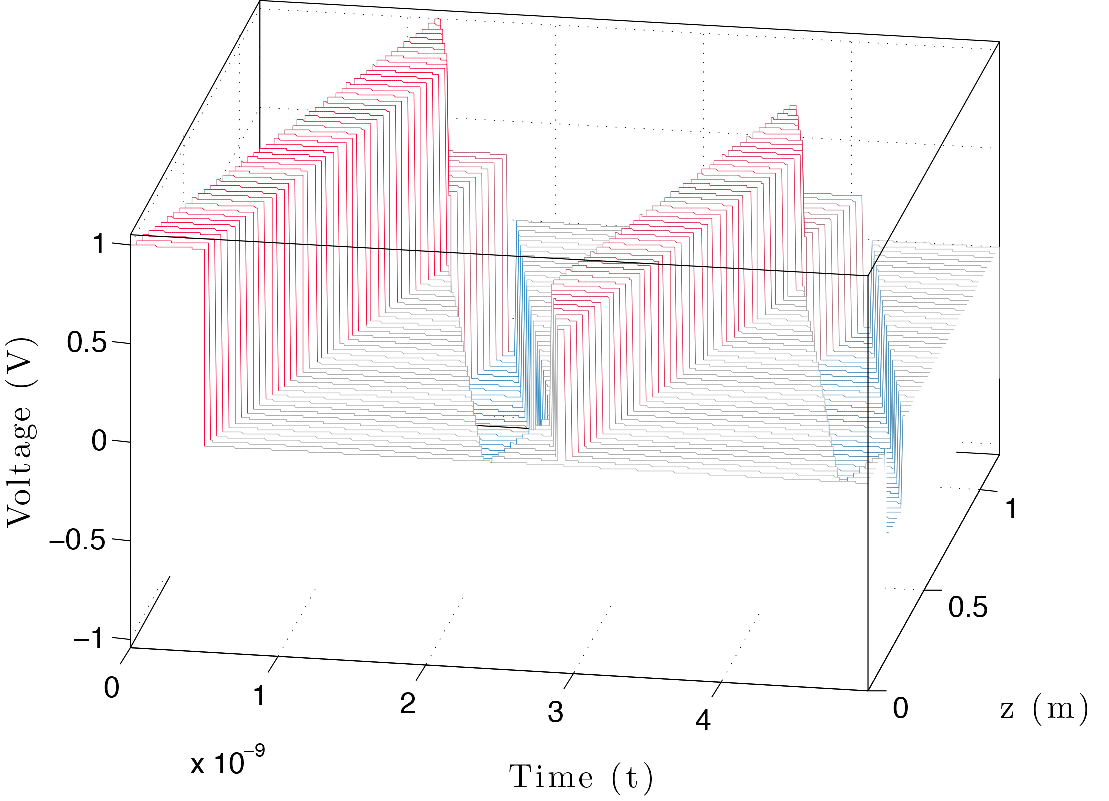
\includegraphics[width=.85\linewidth]{resource/voltage-cropped.pdf}
	\caption{Space-time plot of the voltage across the channel}
	\label{fig:ass-1-v}
\end{figure}
\begin{figure}[H]
	\centering
	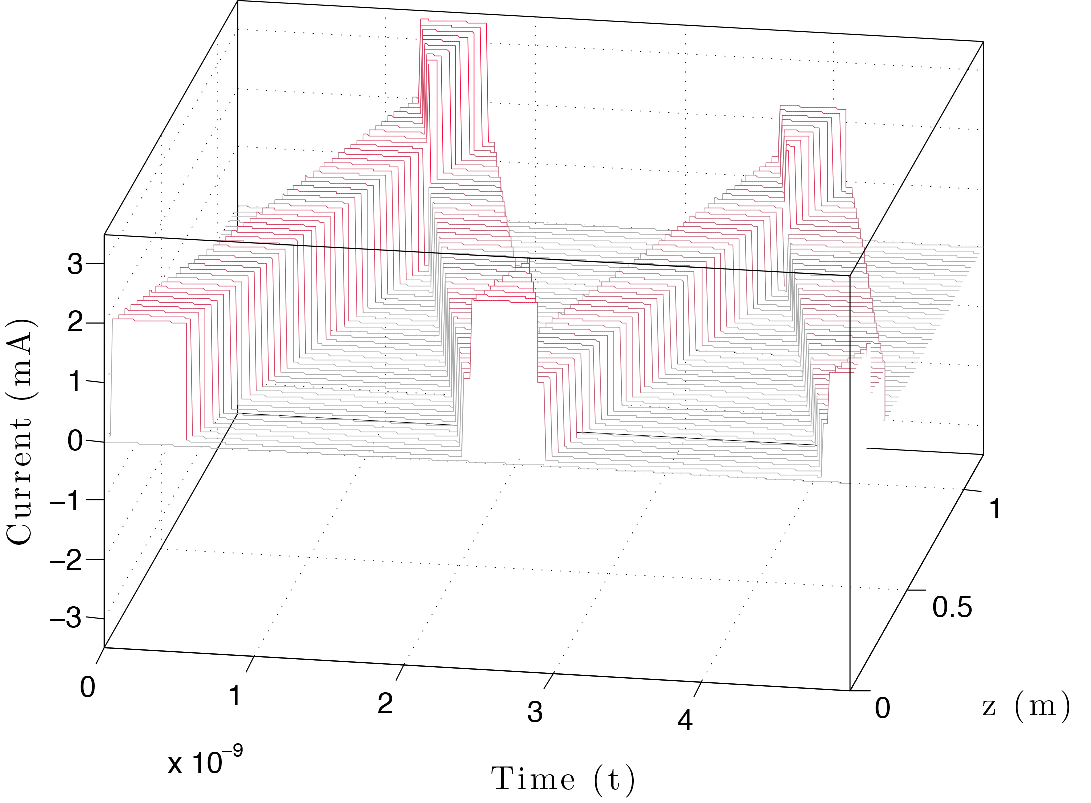
\includegraphics[width=.85\linewidth]{resource/current-cropped.pdf}
	\caption{Space-time plot of the current across the channel}
	\label{fig:ass-1-i}
\end{figure}

Figure \ref{fig:ass-1-v} and \ref{fig:ass-1-i} show space-time plots of the voltage and derived current across the channel for the parameters given in Table \ref{tab:ass-1-parms}.

\begin{table}[H]
	\centering
	\caption{Parameters used in the space-time plots}
	\label{tab:ass-1-parms}
	\begin{tabular}{c c}
		\hline\hline
		Parameter & Value \\
		\hline
		$V_{\text{max}}$ & \SI{1}{V} \\
		$t_w$ & \SI{0.5}{ns} \\
		$L$ & \SI{0.5}{$\mu$H} \\
		$C$ & \SI{2}{pF} \\
		$Z_l$ & \SI{100}{$\Omega$} \\
		\hline
	\end{tabular}
\end{table}

\section{Task 4}
Let us investigate the transmission channel from Task 2, which is now terminated by a load $Z_l=50+50j$. The reflection coefficient is given by

\begin{equation}
	\Gamma = \frac{Z_l - Z_0}{Z_l + Z_0}.
\end{equation}

As both $Z_l$ and $Z_0$ are frequency-independent, $\Gamma$ is also frequency-independent. Let the voltage at the load be defined by $y(t)$. The normalized power transferred to the load is then given by

\begin{align}
	P_l &= \lim_{T \to \infty} \frac{1}{T} \int_{-T/2}^{T/2} |y(t)|^2 dt, \label{eq:ass-1-esd-lim} \\
	&= \int_{-\infty}^{\infty} \lim_{T \to \infty} \frac{|Y(f)|^2}{T} df \quad \quad \text{(Parseval's theorem),} \nonumber \\
	&= \int_{-\infty}^{\infty} P(f) df.
\end{align}

We are dealing with a time limited signal. This means that $E[y(t)^2]=0$. Therefore it makes sense to discuss the signal's energy instead of power. The ESD of a signal is derived in a same manner as the PSD.

\begin{align}
	E_l &= \lim_{T \to \infty} \int_{-T/2}^{T/2} |y(t)|^2 dt, \label{eq:ass-1-psd-lim} \\
	&= \int_{-\infty}^{\infty} |Y(f)|^2 df \quad \quad \text{(Parseval's theorem),} \nonumber \\
	&= \int_{-\infty}^{\infty} E(f) df.
\end{align}

\begin{figure}[H]
	\centering
	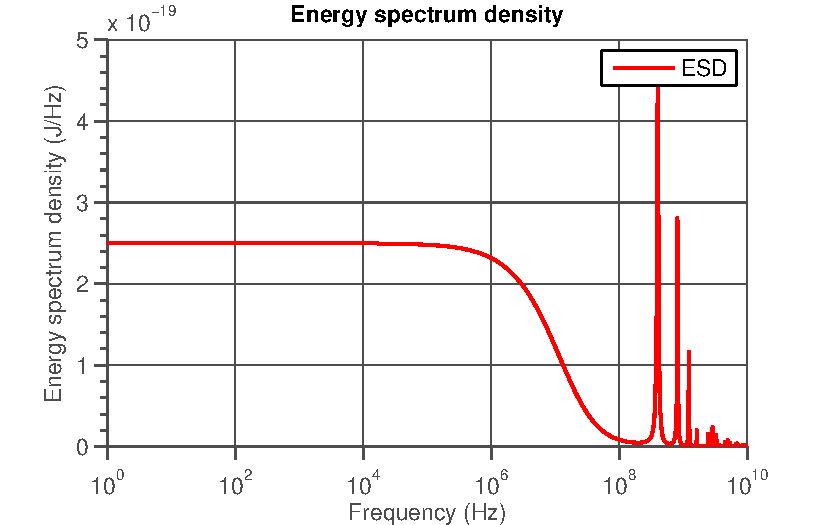
\includegraphics[width=.85\linewidth]{resource/esd.pdf}
	\caption{ESD of $y(t)$}
	\label{fig:ass-1-esd}
\end{figure}

Figure \ref{fig:ass-1-esd} shows the ESD of $y(t)$. We notice that the channel acts as a low-pass filter. We are also able to guess the cutoff frequency by inspecting the graph. This frequency does not match the cutoff frequency $w_0=1/2\sqrt{LC}$ as the channel is not terminated by its characteristic impedance. Furthermore, we inspect interesting behaviour around $f\approx 10^9 \text{ Hz}$.

\begin{figure}[H]
	\centering
	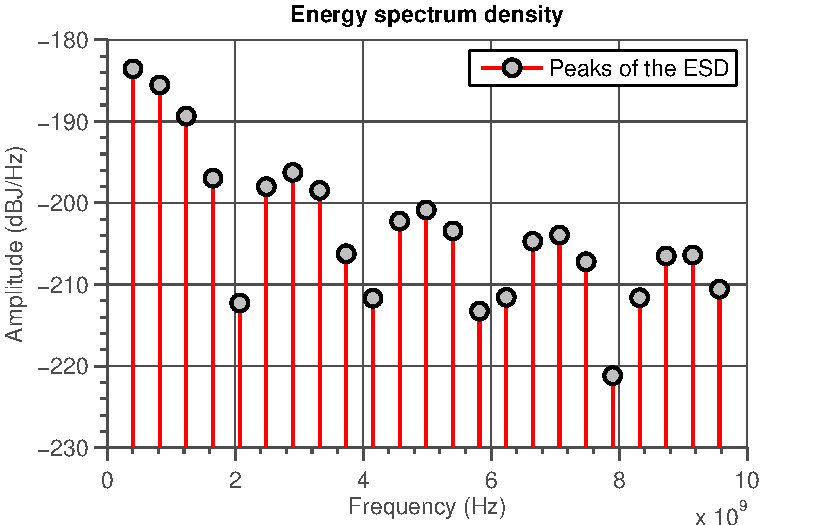
\includegraphics[width=.85\linewidth]{resource/peaks.pdf}
	\caption{Peaks of the ESD of $y(t)$}
	\label{fig:ass-1-peaks}
\end{figure}

Figure \ref{fig:ass-1-peaks} shows the peaks of Figure \ref{fig:ass-1-esd}. We inspect that these peaks are equally spaced! These peaks make us suspect that they belong to standing waves. By assuming that the first peak corresponds with the fundamental frequency, we are able to calculate $\gamma$. The actual $\gamma$ is given by $1.00 \cdot 10^{-9}$. We calculated $\gamma$ also $1.00 \cdot 10^{-9}$. As our calculation matches the actual value very well, we can conclude that our assumption about the standing waves is very likely correct.

We can interpret these peaks in another way. The load at the end of the channel can be considered an anti-node in the case of standing waves. The amplitude swing of the signal is the largest at anti-nodes. We expect therefore that the frequencies which contain the most energy, correspond with standing waves.

We can approximate the energy transferred by approximating the limit in Equation \ref{eq:ass-1-esd-lim}. Approximating yields an input energy of $4.99 \cdot 10^{-10} \text{ J}$. The actual energy of the input signal is given by $V_{\text{max}}^2 t_w =5 \cdot 10^{-10} \text{ J}$. This confirms our method of calculation. In a same manner is the output energy approximated by $1.35 \cdot 10^{-10} \text{ J}$. This yields an efficiency of $\eta\approx0.27$.

\end{document}